\chapter{Estándar CubeSat y especificación CDS}\label{cap:cds}

Este capítulo resume la \emph{CubeSat Design Specification} (CDS), Rev.~14.1, el documento que define las características físicas, eléctricas y operativas de un CubeSat. El objetivo es identificar qué restricciones impone el estándar al transponder de este proyecto, en particular a la cadena de amplificación y a la placa que la contiene. Salvo indicación contraria, los números de sección, valores y tablas citados provienen de la CDS~\cite{cds14}.

%--------------------------------------------------------------------
\section{Origen, propósito y alcance del estándar}\label{sec:cds-general}

El proyecto CubeSat nació en 1999 como una colaboración entre el Prof.~Jordi Puig-Suari (Cal Poly, San Luis Obispo) y el Prof.~Bob Twiggs (Laboratorio de Desarrollo de Sistemas Espaciales de Stanford). Buscaba reducir el costo y el tiempo de desarrollo, facilitar el acceso al espacio y sostener una alta frecuencia de lanzamientos~\cite[Sec.~1.1]{cds14}.

Un CubeSat es un satélite que adopta un tamaño y un factor de forma estandarizados, cuya unidad se denomina <<U>>. Un CubeSat de 1U es un cubo de \SI{10}{\centi\metre} de lado con una masa de hasta \SI{2}{\kilo\gram}~\cite[Sec.~1.1]{cds14}. El estándar cubre configuraciones de 1U a 12U y, como objetivo secundario, informa sobre los dispensadores (desplegadores) disponibles y sus interfaces.

La Rev.~14 (julio de 2020) reemplazó a la Rev.~13 y a la CDS de 6U, incorporó las configuraciones de 6U y 12U y pasó de un conjunto de requisitos rígidos a un documento más cercano a una guía de diseño. La Rev.~14.1 (febrero de 2022) eliminó la marca de borrador, actualizó la información de dispensadores y agregó aclaraciones en las secciones~2 y~3~\cite{cds14,cdsanuncio}. Según el sitio del programa CubeSat, la Rev.~14.1 es la versión vigente~\cite{cubesatinfo}.

\subsection{Jerarquía normativa y lenguaje de la especificación}\label{subsec:cds-jerarquia}

Los requisitos de la CDS están pensados para el diseño preliminar y se redactan de forma conservadora, para maximizar la compatibilidad con cualquier vehículo de lanzamiento. Una vez que el satélite está asignado a un lanzamiento, los requisitos del proveedor de lanzamiento (\emph{Launch Provider}) prevalecen sobre los de la CDS\@. Aun así, un diseño que cumpla la CDS debería cumplir la mayoría de los requisitos de los proveedores, y cada desvío reduce las posibilidades de encontrar una oportunidad de lanzamiento~\cite[Secs.~1.3 y 1.4]{cds14}.

La CDS distingue cuatro términos en sus especificaciones~\cite[Sec.~1.6]{cds14}:
\begin{itemize}
  \item \textbf{Shall} (<<deberá>>): requisito obligatorio, sujeto a verificación formal.
  \item \textbf{Should} (<<debería>>): recomendación fuerte. No cumplirla suele limitar las oportunidades de lanzamiento.
  \item \textbf{Will} (<<ocurrirá>>): evento que sucederá independientemente del desarrollador, y para el cual este debe estar preparado.
  \item \textbf{Note} (<<nota>>): consejo orientativo.
\end{itemize}

%--------------------------------------------------------------------
\section{Configuraciones y el CubeSat 1U}\label{sec:cds-configuraciones}

La Tabla~\ref{tab:cds-masa-cg} resume la masa típica máxima y los rangos admisibles del centro de gravedad (CG) para cada configuración, medidos desde el centro geométrico~\cite[Sec.~2.2.10 y 2.2.11, Tablas~1 y~2]{cds14}. La CDS aclara que se pueden evaluar masas mayores caso por caso, y que la masa admisible depende de las capacidades del dispensador.

\begin{table}[H]
  \centering
  \caption[Masa y centro de gravedad por configuración (CDS Rev.~14.1)]{Masa típica máxima y rango admisible del centro de gravedad por configuración (CDS Rev.~14.1, Tablas~1 y~2).}\label{tab:cds-masa-cg}
  \setlength{\tabcolsep}{5pt}
  \begin{tabular}{lcccc}
    \toprule
    Configuración & Masa [\si{\kilo\gram}] & X [\si{\centi\metre}] & Y [\si{\centi\metre}] & Z [\si{\centi\metre}] \\
    \midrule
    1U   & 2,00  & $\pm 2$   & $\pm 2$   & $\pm 2$   \\
    1,5U & 3,00  & $\pm 2$   & $\pm 2$   & $\pm 3$   \\
    2U   & 4,00  & $\pm 2$   & $\pm 2$   & $\pm 4{,}5$ \\
    3U   & 6,00  & $\pm 2$   & $\pm 2$   & $\pm 7$   \\
    6U   & 12,00 & $\pm 4{,}5$ & $\pm 2$ & $\pm 7$   \\
    12U  & 24,00 & $\pm 4{,}5$ & $\pm 4{,}5$ & $\pm 7$ \\
    \bottomrule
  \end{tabular}
\end{table}

Para el 1U, la masa máxima es de \SI{2}{\kilo\gram} y el CG debe quedar dentro de una caja de $\pm\SI{2}{\centi\metre}$ en cada eje. Esto es relevante para el diseño de la placa: la distribución de masas (batería, placas apiladas, PA con su disipador) afecta directamente el CG del satélite completo.

% Sugerencia: agregar en Figuras/ el dibujo del 1U del Apéndice B de la CDS y la Figura 2 (familia CubeSat).
% \begin{figure}[H]
%   \centering
%   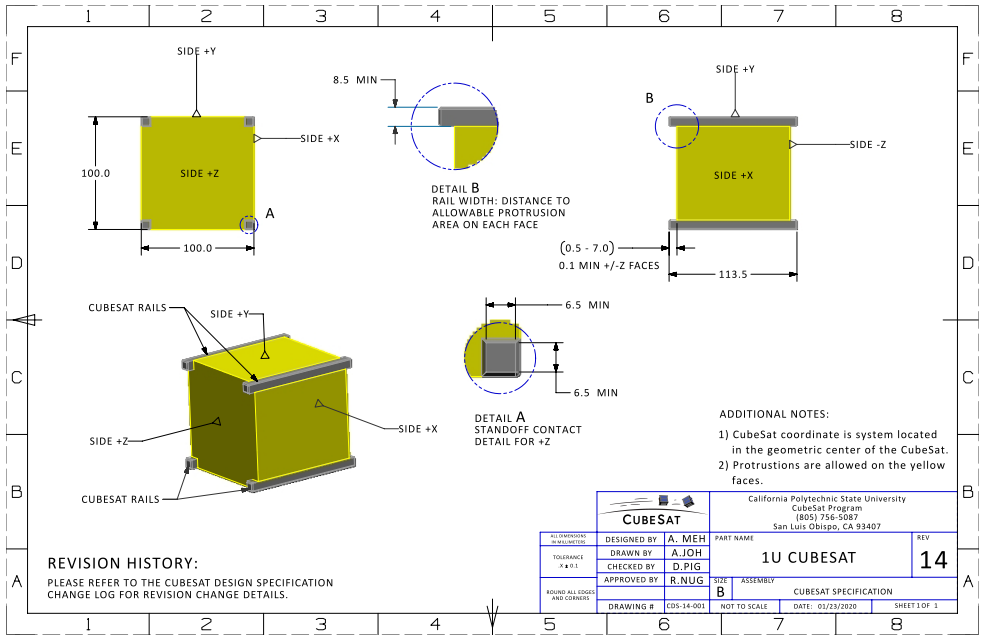
\includegraphics[width=0.8\textwidth]{cds_1u_dibujo.png}
%   \caption{Dibujo de especificación del CubeSat 1U (CDS Rev.~14.1, Apéndice~B)~\cite{cds14}.}
%   \label{fig:cds-1u}
% \end{figure}

%--------------------------------------------------------------------
\section{Especificaciones generales}\label{sec:cds-generales}

La sección~2.1 de la CDS reúne requisitos de seguridad y compatibilidad aplicables a todo el satélite~\cite[Sec.~2.1]{cds14}:

\begin{itemize}
  \item \textbf{Integridad:} ninguna parte puede desprenderse del satélite durante el lanzamiento, la eyección o la operación (2.1.1).
  \item \textbf{Pirotecnia, propulsión y materiales peligrosos:} deben cumplir el manual de seguridad de rango AFSPCMAN~91\nobreakdash-710, Vol.~3 (2.1.2, 2.1.3 y 2.1.6). Los sistemas de propulsión requieren al menos tres inhibiciones de activación (2.1.4). Este proyecto no incluye propulsión.
  \item \textbf{Baterías:} se recomienda considerar los límites de la FAA para baterías transportadas por pasajeros; por ejemplo, \SI{100}{\watt\hour} por batería de ion-litio de consumo (2.1.5).
  \item \textbf{Desgasificación (\emph{outgassing}):} los materiales deben tener una pérdida total de masa (TML) $\leq \SI{1,0}{\percent}$ y una masa volátil condensable colectada (CVCM) $\leq \SI{0,1}{\percent}$ (2.1.7). La CDS remite a la base de datos de materiales de la NASA\@.
  \item \textbf{Campo magnético:} los imanes pasivos deben limitar su campo a 0{,}5~gauss por encima del campo terrestre, fuera de la envolvente estática del satélite (2.1.8).
  \item \textbf{Venteo durante el ascenso:} el satélite debe admitir el venteo de ascenso con una relación volumen ventilable/área menor a \SI{50,8}{\metre} (2000 pulgadas) (2.1.9).
\end{itemize}

%--------------------------------------------------------------------
\section{Especificaciones mecánicas}\label{sec:cds-mecanicos}

Las dimensiones y características mecánicas se definen en los dibujos del Apéndice~B de la CDS\@. La CDS sugiere usar el procedimiento CIFP (\emph{CubeSat Inspection and Fit-check Procedure}), publicado en cubesat.org, para verificar el cumplimiento dimensional. Los requisitos de esta sección aplican a dispensadores que no usan el método de sujeción por pestañas (\emph{tabs}); los CubeSats con pestañas tienen requisitos propios, publicados por Planetary Systems Corporation (PSC)~\cite[Sec.~2.2]{cds14}.

\subsection{Sistema de coordenadas y dimensiones}\label{subsec:cds-coordenadas}

El origen del sistema de coordenadas está en el centro geométrico del CubeSat, y las dimensiones deben ajustarse al apartado correspondiente del Apéndice~B (2.2.1 y 2.2.1.1). La cara $-Z$ se inserta primero en el dispensador (2.2.2). Los separadores (\emph{standoffs}) de las caras $\pm Z$ evitan la interferencia con satélites vecinos y con la interfaz del dispensador (2.2.1.2)~\cite{cds14}.

Los valores dimensionales exactos del 1U (lado, altura total, tolerancias, posición de los rieles) están en el dibujo del Apéndice~B. \verificar{transcribir las cotas del 1U directamente del dibujo del Apéndice B de la CDS Rev.~14.1; el texto extraído no las incluye}

\subsection{Rieles y protuberancias}\label{subsec:cds-rieles}

\begin{itemize}
  \item Ningún componente de las caras laterales indicadas en el Apéndice~B puede sobresalir más de \SI{6,5}{\milli\metre} del plano del riel (2.2.3).
  \item Los elementos desplegables deben ser retenidos por el CubeSat y no por el dispensador (2.2.4).
  \item Los rieles deben tener un ancho mínimo de \SI{8,5}{\milli\metre}, medido desde el borde del riel hasta la primera protuberancia de cada cara (2.2.5).
  \item Los rieles deberían tener una rugosidad superficial menor a \SI{1,6}{\micro\metre} (2.2.6), lo que normalmente se cumple con un anodizado correcto, y sus bordes deberían estar redondeados con un radio de al menos \SI{1}{\milli\metre} (2.2.7).
  \item Los extremos de los rieles en las caras $\pm Z$ deben ofrecer una superficie de contacto mínima de $\SI{6,5}{\milli\metre} \times \SI{6,5}{\milli\metre}$ con los rieles de satélites vecinos (2.2.8). Si el CubeSat no comparte dispensador, el proveedor de lanzamiento puede eximir este requisito (2.2.8.1).
  \item Al menos el \SI{75}{\percent} del largo del riel debería estar en contacto con los rieles del dispensador; el \SI{25}{\percent} puede estar rebajado (2.2.9).
\end{itemize}

\subsection{Materiales y tratamiento superficial}\label{subsec:cds-materiales}

La estructura del CubeSat debería ser de aleación de aluminio. Típicamente se usan las aleaciones 7075, 6061, 6082, 5005 o 5052 tanto en la estructura como en los rieles (2.2.12). Las superficies externas de aluminio que contactan los rieles del dispensador (rieles y separadores) deben tener anodizado duro, para evitar la soldadura en frío dentro del dispensador (2.2.13)~\cite{cds14}.

\subsection{Mecanismo de separación}\label{subsec:cds-separacion}

Si el CubeSat comparte dispensador con otros, cada uno debe tener un mecanismo que favorezca la separación de sus vecinos (2.2.14). Como guía, la CDS recomienda un resorte de separación con fuerza máxima menor a \SI{6,7}{\newton} (1,5~lbf) y carrera mayor a \SI{2,5}{\milli\metre} (0,1~pulgadas). Un resorte demasiado fuerte puede superar al resorte del dispensador y producir una separación impredecible; uno demasiado débil puede no alcanzar a separarlos lo suficiente (2.2.14.1). El mecanismo no debe sobresalir del nivel del separador en configuración estibada (2.2.14.2) y no es necesario si el satélite no comparte dispensador (2.2.14.4)~\cite{cds14}.

%--------------------------------------------------------------------
\section{Especificaciones eléctricas}\label{sec:cds-electricos}

La sección~2.3 define las características de seguridad eléctrica que deben cumplirse con cualquier dispensador~\cite[Sec.~2.3]{cds14}.

\subsection{Estado apagado y conmutador de despliegue}\label{subsec:cds-despliegue}

El sistema de potencia del CubeSat debe estar apagado desde la entrega al vehículo de lanzamiento hasta el despliegue en órbita (2.3.1), de modo de impedir la activación de funciones alimentadas. Esas funciones incluyen subsistemas como el procesamiento y manejo de datos (C\&DH), la comunicación por RF, la determinación y control de actitud y la actuación de mecanismos desplegables. El sistema de potencia incluye las baterías y las celdas solares (2.3.1.1).

El satélite debe tener al menos un conmutador de despliegue (\emph{deployment switch}) que esté accionado mientras el satélite está integrado en el dispensador (2.3.2). En estado accionado debe desconectar eléctricamente el sistema de potencia de las funciones alimentadas (2.3.2.1) y debería quedar al nivel de la superficie externa o por debajo, para no dañar la superficie de contacto (2.3.2.3). Si el conmutador pasa de accionado a liberado y vuelve a accionarse, el satélite debe reiniciarse al estado previo al lanzamiento, incluidos los temporizadores de transmisión y despliegue (2.3.2.4)~\cite{cds14}.

\subsection{Relojes de tiempo real, pin RBF y baterías}\label{subsec:cds-rbf}

\begin{itemize}
  \item \textbf{RTC:} se permiten relojes de tiempo real si cumplen lo anterior, están aislados del sistema de potencia principal, operan a menos de \SI{320}{\kilo\hertz} y tienen la corriente limitada a menos de \SI{10}{\milli\ampere} (2.3.3).
  \item \textbf{Pin RBF (\emph{Remove Before Flight}):} el satélite debe incluir un pin que corte toda la alimentación mientras esté insertado (2.3.5). Debe sobresalir como máximo \SI{6,5}{\milli\metre} de la superficie del riel (2.3.5.2). Si el dispensador no tiene puertos de acceso, el RBF debe retirarse antes de la integración (2.3.5.1), por lo que conviene considerar esto en la secuencia de encendido y arranque (2.3.4.1).
  \item \textbf{Baterías:} el satélite debe incorporar protección de circuito para carga y descarga, que evite el desbalance de celdas. Las celdas modificadas o sin certificación UL requieren documentación y ensayos adicionales (2.3.6).
\end{itemize}

\subsection{Inhibiciones de RF y de desplegables}\label{subsec:cds-inhibiciones}

Este apartado es el más relevante para un transponder. La CDS exige \textbf{al menos tres inhibiciones independientes} para impedir una transmisión de RF involuntaria (2.3.7). Una inhibición es un dispositivo físico entre una fuente de energía y un peligro, y un temporizador \emph{no} cuenta como inhibición independiente (2.3.7.1 y 2.3.7.2). Algunos proveedores de lanzamiento solo exigen una o dos según la potencia de RF de salida, pero la CDS recomienda fuertemente usar tres, porque reduce la documentación y los análisis requeridos (2.3.7.3). De forma análoga, se exigen al menos tres inhibiciones independientes para impedir la liberación involuntaria de estructuras desplegables, como antenas o paneles solares (2.3.8)~\cite{cds14}.

%--------------------------------------------------------------------
\section{Especificaciones operativas}\label{sec:cds-operativos}

La sección~2.4 recoge obligaciones legales y de seguridad hacia otros satélites~\cite[Sec.~2.4]{cds14}:

\begin{itemize}
  \item \textbf{Licencias de radiofrecuencia:} los operadores deben obtener y documentar las licencias de uso de frecuencias (2.4.1). Para frecuencias de radioaficionados se requiere la coordinación de frecuencias de la IARU (2.4.1.1). Además, el satélite debe cumplir los acuerdos y restricciones de licencias de radio de su país, y la CDS remite a la UIT para determinar las aprobaciones necesarias (2.4.2).
  \item \textbf{Escombros orbitales:} el diseño debe ser conforme a NPR~8715.6 (2.4.3). Cualquier componente que reingrese debe hacerlo con una energía menor a \SI{15}{\joule} (2.4.3.1).
  \item \textbf{Temporización post-despliegue:} los desplegables deben esperar al menos \SI{30}{\minute} tras la activación de los conmutadores de despliegue (2.4.4). El satélite no debe generar ni transmitir ninguna señal antes de \SI{45}{\minute} desde el despliegue en órbita (2.4.5), aunque puede encenderse inmediatamente después del despliegue (2.4.5.1).
  \item \textbf{Verificación de ajuste:} se realizan al menos una verificación de encaje (\emph{fit check}) y otra final antes de la integración al dispensador (2.4.7).
\end{itemize}

%--------------------------------------------------------------------
\section{Requisitos de ensayo}\label{sec:cds-ensayos}

La CDS indica que los niveles y requisitos de ensayo son específicos de cada misión y los define el proveedor de lanzamiento. Típicamente se realizan ensayos de vibración aleatoria, de horneado en vacío térmico (\emph{thermal vacuum bakeout}) para asegurar la desgasificación de componentes, de choque (normalmente no requerido para CubeSats) y una inspección visual con mediciones críticas según el CIFP~\cite[Sec.~3]{cds14}. Si el entorno del lanzador se desconoce, pueden usarse como referencia GSFC-STD-7000A y SMC-S-016, aunque sus niveles no garantizan cubrir todos los lanzadores. El satélite puede pasar por una campaña de calificación o de \emph{protoflight}; en este último caso, el modelo de vuelo no debe desarmarse ni modificarse después del ensayo (3.5)~\cite{cds14}.

La CDS \emph{no} fija niveles numéricos de vibración ni de choque: remite al proveedor de lanzamiento. Esto es importante para el diseño de la placa (componentes pesados, sujeción de conectores, fijación del PA), porque los niveles reales se conocerán recién al definirse el lanzamiento.

%--------------------------------------------------------------------
\section{Dispensadores}\label{sec:cds-dispensadores}

El dispensador lleva los CubeSats y es la interfaz con el vehículo de lanzamiento. Todos los dispensadores actuales adhieren a uno de dos sistemas de sujeción: el de \textbf{rieles}, desarrollado por Cal Poly para el P-POD, y el de \textbf{pestañas}, desarrollado por PSC\@. En ambos casos, un resorte impulsa una placa empujadora que eyecta al satélite. La CDS aclara que no se espera que un mismo CubeSat sea compatible con ambos tipos~\cite[Sec.~4]{cds14}.

La CDS lista, en su Tabla~3, los dispensadores disponibles (P-POD, ISIPOD, 6-POD, QuadPack, J-SSOD, CSD de PSC, NLAS de Tyvak, entre otros) con sus opciones: puertos de acceso, masa adicional, longitud extendida, protuberancias extendidas, puerto de energía/datos, purga gaseosa y volumen adicional en $-Z$ (\emph{tuna can})~\cite[Sec.~5]{cds14}. Advierte además que diseñar el satélite para una característica que no está en todos los dispensadores restringe las oportunidades de lanzamiento.

%--------------------------------------------------------------------
\section{Implicancias para el transponder}\label{sec:cds-implicancias}

La Tabla~\ref{tab:cds-impacto} relaciona las especificaciones de la CDS con las decisiones de diseño de la cadena de amplificación y de la placa del transponder. La columna de impacto es una interpretación de este trabajo, no un requisito de la CDS\@.

\begin{table}[H]
  \centering
  \caption[Especificaciones de la CDS con impacto sobre el transponder]{Especificaciones de la CDS con impacto sobre el transponder (la columna <<Impacto>> es una interpretación propia).}\label{tab:cds-impacto}
  \small
  \begin{tabular}{@{}>{\raggedright\arraybackslash}p{2.2cm}>{\raggedright\arraybackslash}p{5.6cm}>{\raggedright\arraybackslash}p{7.2cm}@{}}
    \toprule
    Sección & Contenido & Impacto sobre el diseño \\
    \midrule
    2.3.7 & Al menos tres inhibiciones de RF independientes; un temporizador no cuenta. & Prever un mecanismo físico que corte la alimentación o la señal de la cadena de amplificación. Definir con el equipo de sistema cuáles inhibiciones recaen en este subsistema. \\
    2.3.1 y 2.3.2 & Sistema apagado hasta el despliegue; conmutador que desconecta la potencia de las funciones alimentadas. & El transponder no debe quedar alimentado con el conmutador accionado. Revisar la distribución de alimentación en la placa. \\
    2.4.5 & Sin transmisión hasta \SI{45}{\minute} después del despliegue. & El PA debe permanecer inhibido durante ese período. \\
    2.4.1 y 2.4.2 & Licencia y coordinación de frecuencias (IARU para radioaficionados). & Las bandas de operación (VHF/UHF) y la potencia de salida deben ser consistentes con la licencia que se tramite. \\
    2.1.7 & TML $\leq \SI{1,0}{\percent}$ y CVCM $\leq \SI{0,1}{\percent}$. & Condiciona la elección de sustrato, máscara, adhesivos y componentes. \\
    2.2.10 y 2.2.11 & Masa de hasta \SI{2}{\kilo\gram} y CG dentro de $\pm\SI{2}{\centi\metre}$ en el 1U. & Limita la masa del PA y su disipación, y la ubicación de componentes pesados. \\
    2.2.3 y 2.2.5 & Protuberancias de hasta \SI{6,5}{\milli\metre} y ancho mínimo de riel de \SI{8,5}{\milli\metre}. & Restringe la altura de conectores y componentes que sobresalgan. \\
    2.1.8 & Imanes pasivos limitados a 0{,}5~gauss. & Cuidado con componentes magnéticos (inductores, relés, aisladores/circuladores de ferrita). \\
    3 & Ensayos de vibración y térmico-vacío definidos por el proveedor de lanzamiento. & Elegir componentes y fijaciones aptos para vibración y vacío. \\
    \bottomrule
  \end{tabular}
\end{table}

La CDS no fija un presupuesto de potencia ni tensiones de bus: esos valores dependen del subsistema de energía del satélite que desarrolla la facultad. Tampoco se menciona el estándar PC/104 en el texto de la especificación, de modo que el apilamiento de placas es una decisión de diseño del proyecto, que se estudia en el Capítulo~\ref{cap:pc104}.

%--------------------------------------------------------------------
\section{Síntesis}\label{sec:cds-sintesis}

La CDS Rev.~14.1 define una envolvente mecánica y un conjunto de salvaguardas eléctricas y operativas que cualquier CubeSat debe respetar para ser aceptado en un lanzamiento. Para el transponder del proyecto, los puntos de mayor impacto son las inhibiciones de RF, el retardo de \SI{45}{\minute} para transmitir, la licencia de frecuencias, los límites de masa y de centro de gravedad del 1U, y los criterios de materiales de bajo \emph{outgassing}. Los requisitos del proveedor de lanzamiento prevalecen sobre los de la CDS, por lo que los valores aquí presentados deben tomarse como el punto de partida de diseño.